\section*{
نگاه منطقی
\LTRfootnote{ Logical View}
}

سیستم آجاره شامل ۶ کلاس اصلی است که هر کدام به صورت زیر هستند:

\begin{itemize}

\item \textbf{\lr{User}}
نمایان‌گر هر کاربر در سیستم است. فیلدهای اصلی آن نام کاربری و آدرس ایمیل و رمز عبور هستند.

\item \textbf{\lr{Profile}}
هر کابر یک پروفایل دارد که مابقی اطلاعات اضافی آن از جمله عکس پروفایل و آدرس و غیره داخل آن هتسند.

\item \textbf{\lr{Porduct}}
نمایان‌گر محصول در سیستم است. اجزای اصلی هر محصول عکس، قیمت و توضیحات آن هستند.

\item \textbf{\lr{Order}}
با هر سفارش کاربر برای محصولات یک مدل سفارش ساخته می‌شود که تاریخ سفارش و وضعیت سفارش در آن نگه‌داری می‌شوند.

\item \textbf{\lr{Comment}}
هر کاربر می‌تواند روی پست‌ها کامنت‌گذاری کند که در این مدل ذخیره می‌شوند.

\item \textbf{\lr{Rating}}
هر کاربر می‌تواند به محصولات امتیاز بدهد که در این مدل ذخیره می‌شود.

\end{itemize}

دیاگرام یوام‌ال
\LTRfootnote{ UML}
مدل‌های سیستم در شکل 
\ref{uml}
آمده‌است.

\begin{figure}
\centering
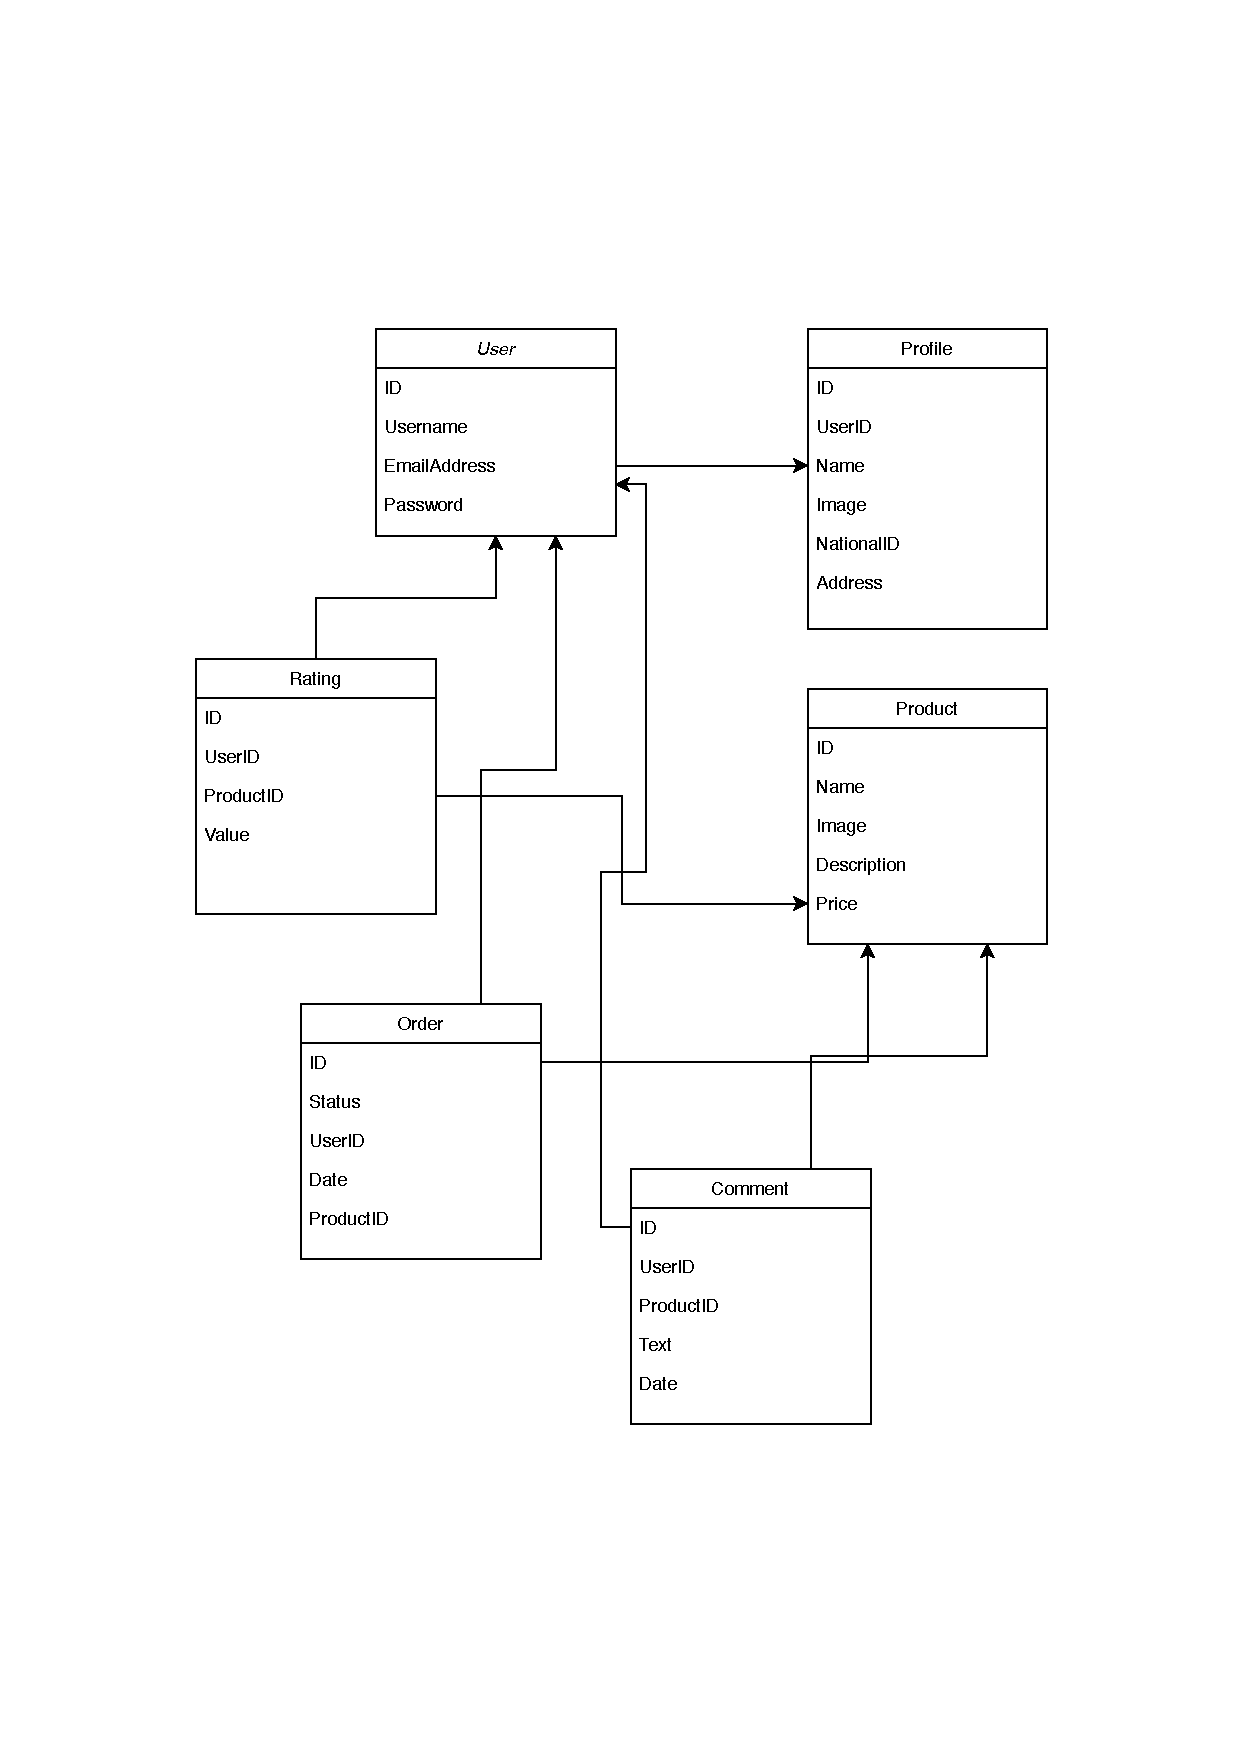
\includegraphics[width=\textwidth]{diagrams/diagram.pdf}
\caption{دیاگرام مدل‌های سیستم}
\label{uml}
\end{figure}

\section*{
نگاه توسعه
\LTRfootnote{ Development View}
}

نگاه توسعه تمرکزش روی سازمان دادن به نرم‌افزار و محیط توسعه آن است. در سیستم‌های بزرگ معمولا بین ۴ تا ۶ لایه توسعه وجود دارد. برای سیستم آجاره ۴ لایه در نظر می‌گیریم:

\begin{itemize}
\item \textbf{سخت‌افزار و سیستم‌عامل}
این لایه مربوط به مدیریت سیستم‌عامل و سخت‌افزار سرورهای موجود برای سیستم آجاره هست. مدیریت میزان منابع و نسخه و کانفیگ سیستم‌عامل مربوط به این لایه است.

\item \textbf{زیرساخت}
این لایه مربوط به زیرساخت‌های لازم برای پروژه از جمله پایگاه‌داده
\LTRfootnote{ Database}
است که انتخاب و نصب و نگه‌داری آن مربوط به این لایه است.

\item \textbf{کاربران و محصولات}
این لایه مربوط به ساخت حساب کاربری برای کاربران و ایجاد محصولات است. کلاس‌ها و عملکردهای مربوط به ثبت‌نام و ورود کابران همچنین ایجاد محصولات در این لایه قرار دارد.

\item \textbf{اجاره و پس‌دادن}
این لایه مربوط به عملیات اجاره دادن و پس‌گرفتن محصولات اجاره داده‌شده است. این لایه‌که به اصطلاح 
\lr{Domain Specific}
است در آخرین لایه قرار دارد.


\end{itemize}

توجه کنید که در این سیستم محتویات هر لایه فقط به لایه‌های قبل از آن وابسته‌اند. همچنین مسئولیت هر لایه با یک نفر است (لایه اول تا چهارم به ترتیب صادق، کیارش، بنیامین و آریو).

